\documentclass[10pt,aspectratio=169]{beamer}

% Compilar con LuaLaTeX (latexmk ya está configurado en .latexmkrc)
\usepackage[spanish,es-tabla,es-nodecimaldot]{babel}
\usepackage{csquotes}

% --- Tema e-ink (Hyprland/Waybar) ---
\usetheme{eink}

% --- Paquetes ---
\usepackage{amsmath,amssymb}
\usepackage{booktabs}
\usepackage{graphicx}
\graphicspath{{figuras/}}
\usepackage{pgfplots}
\usepackage{qrcode}
\pgfplotsset{compat=1.18}

% --- Bibliografía ---
\usepackage[backend=biber,style=numeric]{biblatex}
\addbibresource{referencias.bib}

% Precisión obtenida en el conjunto de prueba (actualizar tras ejecutar el script)
\newcommand{\precision}{95.66\,\%}

\title{Clasificación de automóviles con redes neuronales}
\subtitle{Proyecto 1 --- Conjunto de datos \emph{Car Evaluation}}
\author{Joel Reyes García \and Rodrigo Sosa Mendoza}
\institute{Fundamentos de Inteligencia Artificial}
\date{\today}
\titlegraphic{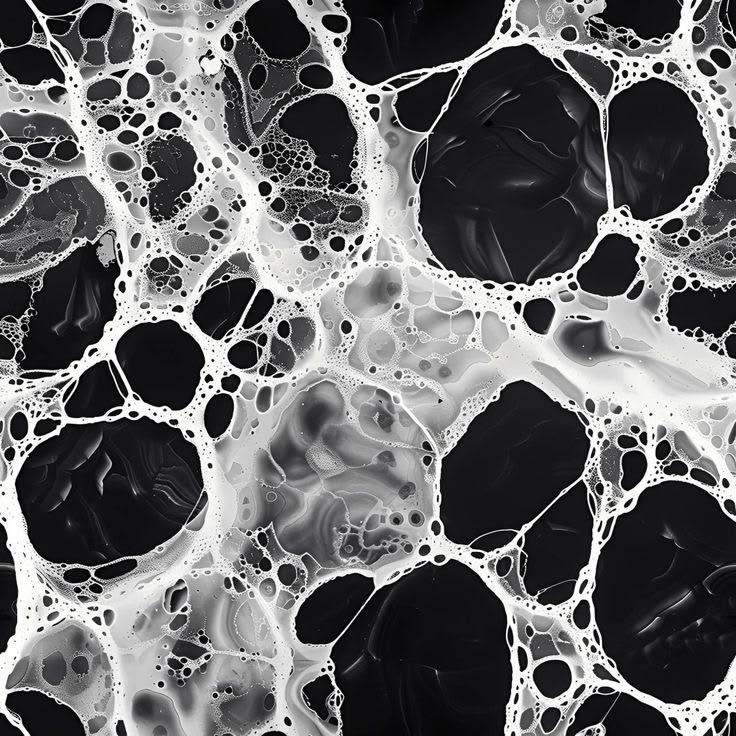
\includegraphics[height=\paperheight]{logo.jpg}}
\piedeportada{Perceptrón multicapa 6 → 32 → 16 → 4}

\begin{document}

\begin{frame}[plain,noframenumbering]
  \titlepage
\end{frame}

% ============================================================
\section{Planteamiento}
% ============================================================

\begin{frame}{Objetivo}
  \begin{itemize}
    \setlength{\itemsep}{0.8em}
    \item Predecir la \alert{aceptabilidad} de un automóvil a partir de sus
          características técnicas y de precio.
    \item Problema de \alert{clasificación multiclase} con 4 categorías.
    \item Modelo: perceptrón multicapa (MLP) con \texttt{TensorFlow/Keras}.
  \end{itemize}

  \vspace{1.2em}
  \centering
  \begin{tikzpicture}[
      cls/.style={draw=ink, line width=\inkthin, fill=paper, minimum width=24mm,
                  minimum height=9mm, font=\bfseries},
    ]
    \foreach \c/\d [count=\i] in {unacc/inaceptable, acc/aceptable, good/bueno, vgood/muy bueno} {
      \fill[ink] ({(\i-1)*30mm+\inkshadow}, -\inkshadow) rectangle ++(24mm,-9mm);
      \node[cls, anchor=north west] at ({(\i-1)*30mm}, 0) {\c};
      \node[font=\scriptsize, text=inactive!60!ink] at ({(\i-1)*30mm+12mm}, -14mm) {\d};
    }
  \end{tikzpicture}
\end{frame}

\begin{frame}{Conjunto de datos}
  \emph{Car Evaluation}, repositorio UCI~\cite{bohanec1988car}:
  \alert{1728 instancias}, 6 atributos categóricos, sin valores faltantes.

  \vspace{1.2em}
  \begin{ventana}[width=0.9\linewidth, before=\centering, left=0mm, right=0mm, top=3mm, bottom=3mm]
    \centering\small
    \renewcommand{\arraystretch}{1.25}
    \setlength{\tabcolsep}{2.5mm}
    \begin{tabular}{lll}
      \textbf{Atributo} & \textbf{Descripción} & \textbf{Valores} \\
      \midrule
      \texttt{buying}    & Precio de compra       & low, med, high, vhigh \\
      \texttt{maint}     & Costo de mantenimiento & low, med, high, vhigh \\
      \texttt{doors}     & Número de puertas      & 2, 3, 4, 5more \\
      \texttt{persons}   & Capacidad de personas  & 2, 4, more \\
      \texttt{lug\_boot} & Tamaño de la cajuela   & small, med, big \\
      \texttt{safety}    & Nivel de seguridad     & low, med, high \\
    \end{tabular}
  \end{ventana}
\end{frame}

\begin{frame}{Distribución de clases}
  \begin{columns}[c]
    \begin{column}{0.56\textwidth}
      \begin{ventana}
        \centering
        \begin{tikzpicture}
          \begin{axis}[
              ybar,
              width=\linewidth, height=5.2cm,
              bar width=20pt,
              ymin=0, ymax=1400,
              symbolic x coords={unacc,acc,good,vgood},
              xtick=data,
              xticklabel style={font=\small\bfseries},
              yticklabel style={font=\scriptsize},
              ylabel={Instancias},
              ylabel style={font=\small},
              nodes near coords,
              nodes near coords style={font=\scriptsize\bfseries},
              axis lines*=left,
              axis line style={ink, line width=\inkthin},
              major tick style={ink},
              enlarge x limits=0.2,
            ]
            \addplot[fill=ink, draw=none] coordinates
              {(unacc,1210) (acc,384) (good,69) (vgood,65)};
          \end{axis}
        \end{tikzpicture}
      \end{ventana}
    \end{column}
    \begin{column}{0.40\textwidth}
      \small
      \begin{tabular}{lr}
        \texttt{unacc} & 70.0\,\% \\
        \texttt{acc}   & 22.2\,\% \\
        \texttt{good}  &  4.0\,\% \\
        \texttt{vgood} &  3.8\,\% \\
      \end{tabular}

      \vspace{1em}
      \alert{Conjunto desbalanceado}\\[0.3em]
      \texttt{good} y \texttt{vgood} son clases minoritarias.
    \end{column}
  \end{columns}
\end{frame}

% ============================================================
\section{Metodología}
% ============================================================

\begin{frame}[fragile]{Preprocesamiento: atributos}
  \begin{columns}[c]
    \begin{column}{0.42\textwidth}
      \small
      \begin{itemize}
        \setlength{\itemsep}{0.5em}
        \item La red solo recibe \textbf{números}, no texto.
        \item Cada atributo tiene un \textbf{orden natural}:
              low < med < high < vhigh.
        \item \textbf{OrdinalEncoder} asigna 0, 1, 2, \dots{} respetando
              ese orden (se le pasa explícito).
      \end{itemize}
    \end{column}
    \begin{column}{0.56\textwidth}
\begin{codigo}{Atributos · OrdinalEncoder}
orden_buying = ["low", "med", "high", "vhigh"]
# ... un orden por cada atributo
ordinal_encoder = OrdinalEncoder(categories=[
    orden_buying, orden_maint, orden_doors,
    orden_persons, orden_lug_boot, orden_safety])
X = ordinal_encoder.fit_transform(X)
# low->0  med->1  high->2  vhigh->3
\end{codigo}
    \end{column}
  \end{columns}

  \vspace{1.2em}
  \textbf{División de los datos} {\small(\texttt{random\_state=42})}
  \vspace{0.6em}

  \centering
  \begin{tikzpicture}[x=0.08mm]
    \fill[ink] (\inkshadow,-\inkshadow) rectangle ++(1728,7mm);
    \fill[ink]   (0,0)    rectangle (1105,7mm) node[midway,text=paper,font=\footnotesize\bfseries] {Entrenamiento · 1105};
    \fill[sage]  (1105,0) rectangle (1382,7mm) node[midway,text=paper,font=\scriptsize\bfseries] {Valid. · 277};
    \fill[paper] (1382,0) rectangle (1728,7mm) node[midway,text=ink,font=\scriptsize\bfseries] {Prueba · 346};
    \draw[ink, line width=\inkthin] (0,0) rectangle (1728,7mm);
    \draw[ink, line width=\inkthin] (1105,0) -- ++(0,7mm) (1382,0) -- ++(0,7mm);
  \end{tikzpicture}
\end{frame}

\begin{frame}[fragile]{Preprocesamiento: etiqueta}
  \begin{columns}[c]
    \begin{column}{0.44\textwidth}
      \small
      \begin{itemize}
        \setlength{\itemsep}{0.6em}
        \item \textbf{LabelEncoder} convierte cada clase en un entero.
        \item Usa \textbf{orden alfabético}:\\
              acc\,=\,0, good\,=\,1, unacc\,=\,2, vgood\,=\,3.
        \item El orden no importa: hay \textbf{una neurona de salida por clase}.
        \item Queda como entero (no \emph{one-hot}); por eso la pérdida es la
              versión \textbf{sparse}.
        \item \textbf{inverse\_transform} regresa la predicción a texto.
      \end{itemize}
    \end{column}
    \begin{column}{0.54\textwidth}
\begin{codigo}{Etiqueta · LabelEncoder}
label_encoder = LabelEncoder()
y = label_encoder.fit_transform(y)

label_encoder.classes_
# ['acc', 'good', 'unacc', 'vgood']
#    0      1       2        3

# Después de predecir: número -> texto
label_encoder.inverse_transform([1])
# ['good']
\end{codigo}
    \end{column}
  \end{columns}
\end{frame}

\begin{frame}{Arquitectura de la red}
  \begin{columns}[c]
    \begin{column}{0.52\textwidth}
      \begin{ventana}
        \centering
        \begin{tikzpicture}[
            neuron/.style={circle, draw=ink, line width=0.6pt, fill=paper,
                           minimum size=8pt, inner sep=0},
            scale=0.85
          ]
          \foreach \x/\n/\lab/\tot in {0/6/Entrada/6, 2/8/Oculta 1/32, 4/6/Oculta 2/16, 6/4/Salida/4} {
            \foreach \i in {1,...,\n}
              \coordinate (n-\x-\i) at (\x, {(\n+1)/2*0.5 - \i*0.5});
            \node[font=\scriptsize\bfseries, align=center] at (\x,-2.75) {\lab\\(\tot)};
          }
          \foreach \a/\na/\b/\nb in {0/6/2/8, 2/8/4/6, 4/6/6/4} {
            \foreach \i in {1,...,\na} \foreach \j in {1,...,\nb}
              \draw[inactive, very thin] (n-\a-\i) -- (n-\b-\j);
          }
          \foreach \x/\n in {0/6, 2/8, 4/6, 6/4}
            \foreach \i in {1,...,\n}
              \node[neuron] at (n-\x-\i) {};
        \end{tikzpicture}
      \end{ventana}
    \end{column}
    \begin{column}{0.44\textwidth}
      \footnotesize
      \begin{tabular}{lrr}
        \textbf{Capa} & \textbf{Neuronas} & \textbf{Parámetros} \\
        \midrule
        Dense · ReLU    & 32 & 224 \\
        Dense · ReLU    & 16 & 528 \\
        Dense · Softmax &  4 &  68 \\
        \midrule
        Total           &    & \alert{820} \\
      \end{tabular}
    \end{column}
  \end{columns}
\end{frame}

\begin{frame}{Funciones de activación y pérdida}
  \begin{tcbraster}[raster columns=3, raster equal height, raster column skip=5mm,
                    raster force size=false,
                    raster every box/.style={valign=center, halign=center}]
    \begin{ventanat}{ReLU · ocultas}
      \( f(x) = \max(0, x) \)
    \end{ventanat}
    \begin{ventanat}{Softmax · salida}
      \( \displaystyle \hat{y}_k = \frac{e^{z_k}}{\sum_{j=1}^{4} e^{z_j}} \)
    \end{ventanat}
    \begin{ventanat}{Pérdida}
      \( \displaystyle \mathcal{L} = -\frac{1}{N} \sum_{i=1}^{N} \log \hat{y}_{i,\,c_i} \)
    \end{ventanat}
  \end{tcbraster}

  \vspace{1.4em}
  \small
  \begin{itemize}
    \setlength{\itemsep}{0.4em}
    \item Softmax convierte la salida en probabilidades que suman 1.
    \item Entropía cruzada categórica \emph{dispersa}: las etiquetas son
          enteros, no vectores \emph{one-hot}.
  \end{itemize}
\end{frame}

\begin{frame}[fragile]{Entrenamiento}
  \begin{columns}[c]
    \begin{column}{0.38\textwidth}
      \begin{itemize}
        \setlength{\itemsep}{0.5em}
        \item Optimizador: \textbf{Adam}
        \item Épocas: \textbf{250}
        \item Tamaño de lote: \textbf{16}
        \item Validación: \textbf{20\,\%} del entrenamiento
        \item Métrica: exactitud
      \end{itemize}
    \end{column}
    \begin{column}{0.58\textwidth}
\begin{codigo}{proyecto\_1.py}
modelo = Sequential([
    Dense(32, activation="relu", input_shape=(6,)),
    Dense(16, activation="relu"),
    Dense(4, activation="softmax"),
])
modelo.compile(optimizer="adam",
               loss="sparse_categorical_crossentropy",
               metrics=["accuracy"])
modelo.fit(X_train, y_train, epochs=250,
           batch_size=16, validation_split=0.2)
\end{codigo}
    \end{column}
  \end{columns}
\end{frame}

% ============================================================
\section{Resultados}
% ============================================================

\begin{frame}{Desempeño en el conjunto de prueba}
  \begin{columns}[c]
    \begin{column}{0.36\textwidth}
      \inkstat{\precision}{exactitud sobre 346 instancias\\no vistas en el entrenamiento}
    \end{column}
    \begin{column}{0.58\textwidth}
      \begin{ventana}[left=1mm, right=1mm, top=1mm, bottom=1mm]
        \centering
        \IfFileExists{figuras/matriz_confusion.png}{%
          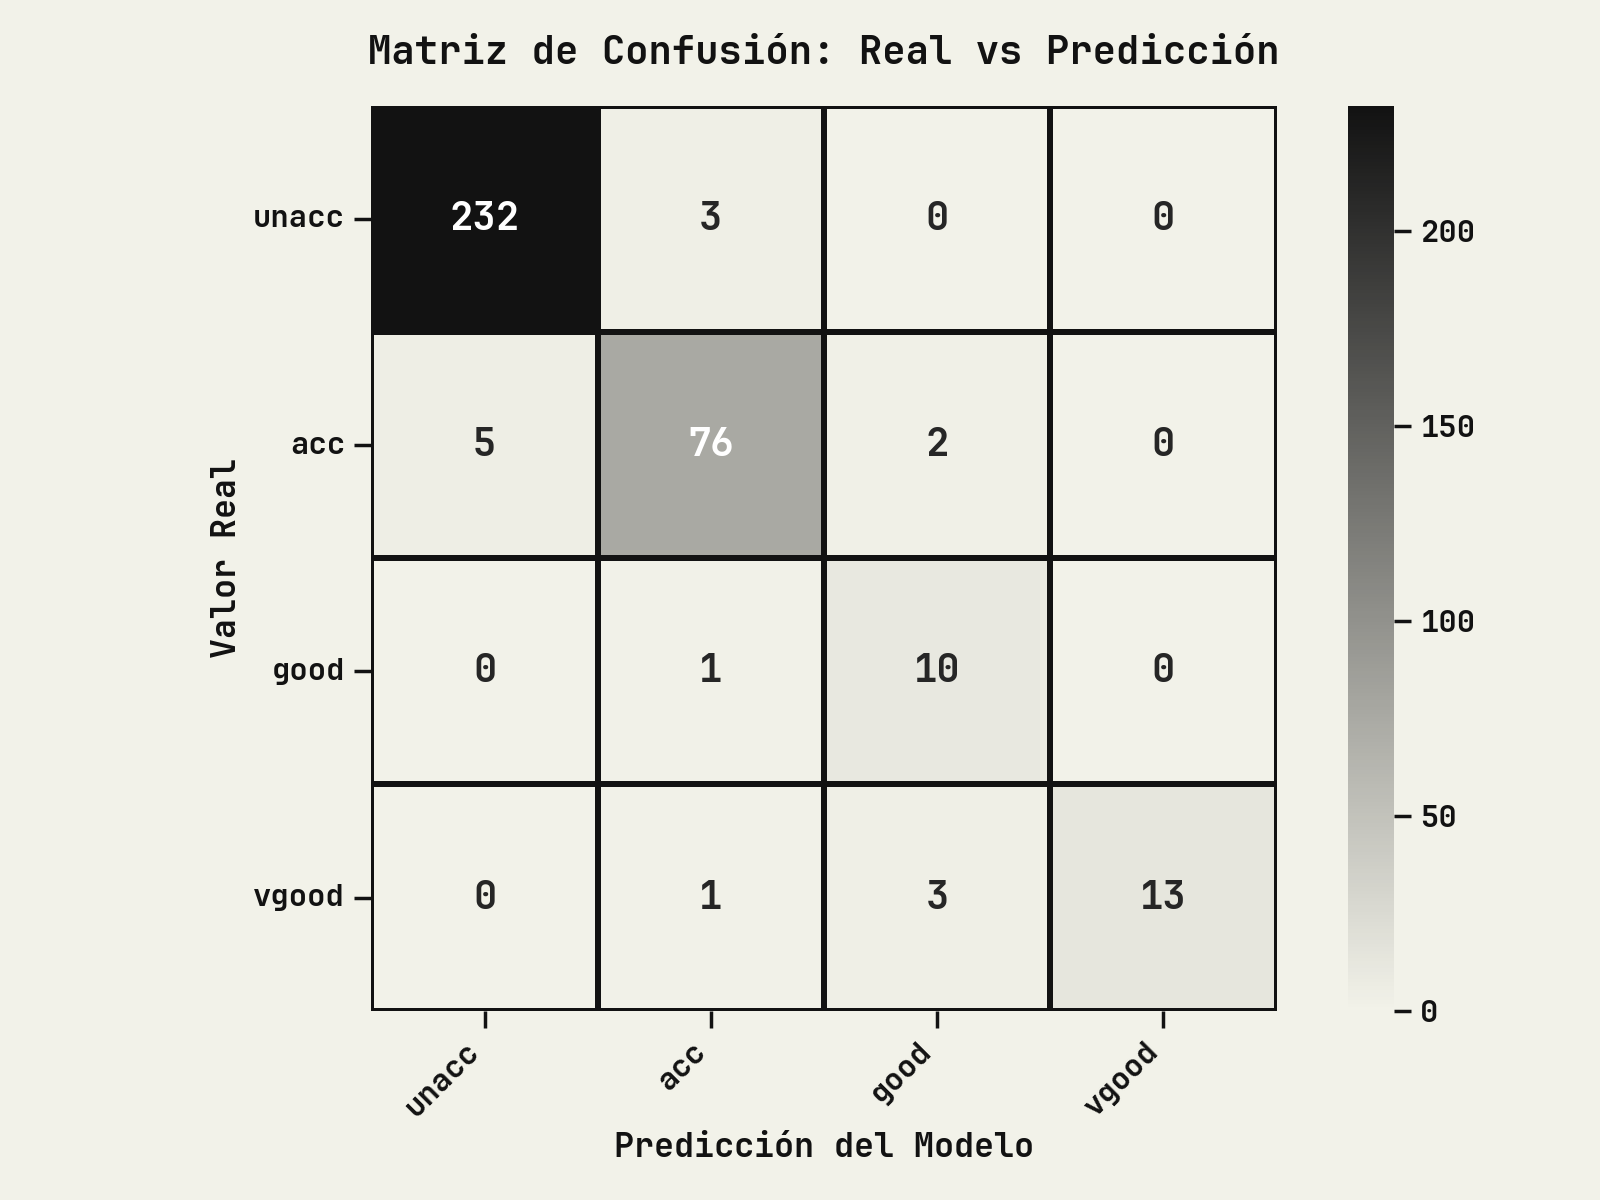
\includegraphics[height=0.66\textheight]{matriz_confusion.png}%
        }{%
          \parbox[c][0.5\textheight][c]{0.9\linewidth}{\centering\footnotesize
            guardar como\\\texttt{figuras/matriz\_confusion.png}}%
        }
      \end{ventana}
    \end{column}
  \end{columns}
\end{frame}

\begin{frame}{Interpretación de la matriz}
  \begin{columns}[c]
    \begin{column}{0.44\textwidth}
      \small
      \begin{itemize}
        \setlength{\itemsep}{0.6em}
        \item \textbf{Filas}: clase real.\\ \textbf{Columnas}: predicción.
        \item \textbf{Diagonal}: aciertos, \alert{331 de 346}.
        \item \textbf{Fuera de la diagonal}: 15 errores.
        \item \textbf{14 de 15} errores son entre clases \textbf{vecinas}
              (\texttt{unacc}↔\texttt{acc}, \texttt{acc}↔\texttt{good},
              \texttt{good}↔\texttt{vgood}).
        \item Nunca confunde \texttt{unacc} con \texttt{good} ni \texttt{vgood}.
      \end{itemize}
    \end{column}
    \begin{column}{0.52\textwidth}
      \begin{ventana}[halign=center]
        \small
        \renewcommand{\arraystretch}{1.2}
        \begin{tabular}{lccc}
          \textbf{Clase} & \textbf{Precisión} & \textbf{Recall} & \textbf{Casos} \\
          \midrule
          unacc & 0.98 & 0.99 & 235 \\
          acc   & 0.94 & 0.92 &  83 \\
          good  & 0.67 & 0.91 &  11 \\
          vgood & 1.00 & 0.76 &  17 \\
        \end{tabular}
      \end{ventana}
      \scriptsize
      \textbf{Precisión}: de lo que predijo como $X$, cuánto era $X$.\\
      \textbf{Recall}: de los $X$ reales, cuántos encontró.
    \end{column}
  \end{columns}
\end{frame}

% ============================================================
\section{Demostración}
% ============================================================

\begin{frame}[fragile]{Guardar el modelo}
  \begin{columns}[c]
    \begin{column}{0.42\textwidth}
      \small
      \begin{itemize}
        \setlength{\itemsep}{0.5em}
        \item Guardar la red evita \textbf{reentrenar} cada vez que se usa.
        \item Se guarda al final del script, después de evaluar.
        \item \textbf{modelo.keras} es un \texttt{.zip} de 35\,KB con la
              arquitectura, los \textbf{820 pesos} y el estado de Adam.
        \item \textbf{No} guarda los encoders: quien lo use debe codificar
              con el mismo orden.
      \end{itemize}
    \end{column}
    \begin{column}{0.56\textwidth}
\begin{codigo}{codigo/proyecto\_1.py}
modelo.fit(X_train, y_train, epochs=250, ...)
modelo.evaluate(X_test, y_test)
modelo.save("app/backend/modelo/modelo.keras")
\end{codigo}
      \begin{ventanat}{Contenido de modelo.keras}
        \footnotesize\hyphenpenalty=10000
        \renewcommand{\arraystretch}{1.1}
        \begin{tabular}{@{}l@{\hspace{3mm}}p{\dimexpr\linewidth-31mm\relax}@{}}
          \textbf{config.json}      & arquitectura 6→32→16→4, activaciones,
                                      pérdida y optimizador \\
          \textbf{model.weights.h5} & los 820 pesos y sesgos + estado de
                                      Adam (17\,500 pasos) \\
          \textbf{metadata.json}    & versión de Keras y fecha \\
        \end{tabular}
      \end{ventanat}
    \end{column}
  \end{columns}
\end{frame}

\begin{frame}[fragile]{Cargar y usar el modelo}
  \begin{columns}[c]
    \begin{column}{0.42\textwidth}
      \small
      \begin{itemize}
        \setlength{\itemsep}{0.5em}
        \item \textbf{load\_model} reconstruye la red con los mismos pesos.
        \item Ya no se entrena: solo la \textbf{pasada hacia adelante}
              (inferencia).
        \item Es lo que hace el backend en cada petición.
      \end{itemize}
      \vspace{1em}
      {\scriptsize\ttfamily proyecto\_1.py → modelo.keras → main.py\par}
    \end{column}
    \begin{column}{0.56\textwidth}
\begin{codigo}{Uso del modelo guardado}
modelo = tf.keras.models.load_model("modelo.keras")

# Auto ya codificado (ver Preprocesamiento)
x = np.array([[0, 1, 3, 2, 1, 1]])

p = modelo(x)[0]
# [0.001, 0.999, 0.000, 0.000]
#   acc   good   unacc  vgood

CLASES[np.argmax(p)]
# 'good'
\end{codigo}
    \end{column}
  \end{columns}
\end{frame}

\begin{frame}[fragile]{Backend con FastAPI}
  \begin{columns}[c]
    \begin{column}{0.38\textwidth}
      \small
      \begin{itemize}
        \setlength{\itemsep}{0.5em}
        \item Carga \textbf{modelo.keras} una vez al arrancar.
        \item Codifica el auto \textbf{igual que en el entrenamiento}.
        \item \textbf{argmax} de las 4 probabilidades da la clase.
        \item \textbf{\textasciitilde10 ms} por predicción;
              \textasciitilde400/s con 4 procesos.
        \item En \textbf{Docker}, solo accesible desde la red interna.
      \end{itemize}
    \end{column}
    \begin{column}{0.60\textwidth}
\begin{codigo}{app/backend/main.py (simplificado)}
modelo = load_model("modelo/modelo.keras")
app = FastAPI()

@app.post("/api/predecir")
def predecir(auto: Auto):
    entrada = [ORDEN[a].index(getattr(auto, a))
               for a in ORDEN]
    salida = modelo(np.array([entrada]))[0]
    return {
        "clase": CLASES[np.argmax(salida)],
        "probabilidades": dict(zip(CLASES, salida)),
    }
\end{codigo}
    \end{column}
  \end{columns}
\end{frame}

\begin{frame}{Pruébalo}
  \vfill
  \centering
  \begin{tikzpicture}
    \node[inner sep=0] (qr) {\textcolor{ink}{\qrcode[height=48mm]{https://fia.jowlab.com/}}};
    \fill[ink] ($(qr.east)+(8mm,-24mm)$) rectangle ++(1.1mm,48mm);
    \node[anchor=west, align=left, inner sep=0, text width=62mm]
      at ($(qr.east)+(15mm,0)$) {%
      {\Large\bfseries Escanea y\\clasifica un auto\par}
      \vskip3.5mm{\rule{\linewidth}{1.6pt}}\vskip3.5mm
      {\large\bfseries fia.jowlab.com}\par
      \vskip4mm
      {\small Elige las características y la red responde en tiempo
       real con la clase y sus probabilidades.}\par};
  \end{tikzpicture}
  \vfill
\end{frame}

% ============================================================
\section{Conclusiones}
% ============================================================

\begin{frame}{Conclusiones}
  \begin{itemize}
    \setlength{\itemsep}{0.8em}
    \item Una red pequeña (\textbf{820 parámetros}) basta para aprender las
          reglas que definen la aceptabilidad de un automóvil.
    \item La codificación ordinal preserva el orden de los atributos y
          simplifica la entrada de la red.
    \item Los errores se concentran entre clases vecinas: la red aprendió
          el orden de las categorías. \texttt{good} y \texttt{vgood} son las
          más débiles (pocos ejemplos por el desbalance).
    \item Con 250 épocas la exactitud de entrenamiento llega a 100\,\% y la
          de validación a 97\,\%: hay que vigilar el sobreajuste.
    \item \textbf{Trabajo futuro:} pesos por clase, \emph{early stopping} y
          validación cruzada.
  \end{itemize}
\end{frame}

\begin{frame}{Referencias}
  \small
  \printbibliography[heading=none]
\end{frame}

\inkfinal{%
  {\Huge\bfseries Gracias}\\[1em]
  {\large ¿Preguntas?}}

\end{document}
